%% ======================================================================
%% Reconstructed LaTeX source of the IEEE QAI 2026 submission (paper 191)
%% Rebuilt from the submitted PDF "IEEE_QAI___Forgetting (6).pdf" (7 pages,
%% anonymised version, the file actually reviewed by the QAI committee).
%%
%% Original template: IEEE conference template (062824). Anonymised for
%% double-blind review. Real author list:
%%   D. Martín-Pérez, F. Rodríguez-Díaz, D. Gutiérrez-Avilés, A. Troncoso,
%%   F. Martínez-Álvarez
%%
%% NOTE (kept on purpose): the Experiment 1 Table II values of this version
%% differ from the per-seed payloads stored in this repository (see README).
%% ======================================================================
\documentclass[conference]{IEEEtran}
\IEEEoverridecommandlockouts

\usepackage{cite}
\usepackage{amsmath,amssymb,amsfonts}
\usepackage{algorithmic}
\usepackage{graphicx}
\usepackage{textcomp}
\usepackage{xcolor}
\usepackage{booktabs}
\usepackage{tikz}
\usetikzlibrary{positioning}
\def\BibTeX{{\rm B\kern-.05em{\sc i\kern-.025em b}\kern-.08em
    T\kern-.1667em\lower.7ex\hbox{E}\kern-.125emX}}

\begin{document}

\title{Cross-Domain Synthetic Pre-Training for Catastrophic Forgetting Mitigation in Quantum Continual Learning}

%% Anonymised at submission time.
\author{No authors given\\No affiliations given}

\maketitle

\begin{abstract}
Hybrid quantum-classical models trained under continual learning settings suffer from Catastrophic Forgetting, in which previously acquired knowledge degrades while the model adapts to new tasks. This work investigates whether cross-domain synthetic pre-training can mitigate this effect without relying on explicit memory mechanisms. To this end, a cross-domain synthetic pre-training methodology is evaluated, where hybrid quantum-classical models are first trained on synthetic Gaussian data before transitioning to sequential image recognition tasks. The study compares three parameterized quantum circuit ans\"atze, namely Strongly Entangling, Basic Entangler, and Tree Tensor Network, under ideal and simulated noise profiles. Results show that synthetic pre-training mitigates catastrophic forgetting, reducing the drop in performance relative to the naive baseline under the evaluated noise profiles. Furthermore, the Strongly Entangling and Tree Tensor Network architectures achieve higher task retention than the Basic Entangler in the evaluated setting. These findings support the use of cross-domain synthetic pre-training as a promising memory-free initialization strategy for Quantum Continual Learning.
\end{abstract}

\begin{IEEEkeywords}
Quantum Transfer Learning, Quantum Neural Network, Quantum Continual Learning, Catastrophic Forgetting
\end{IEEEkeywords}

% ======================================================================
\section{Introduction}
% ======================================================================
The increasing complexity of Quantum Machine Learning (QML) \cite{b1} models brings important challenges in the optimization of parameterized quantum circuits \cite{b2}. Variational Quantum Circuits (VQCs) combine quantum circuit execution with the classical optimization of trainable circuit parameters. However, when these models are trained under continual learning (CL) settings, their performance may degrade due to Catastrophic Forgetting (CF). This phenomenon occurs when knowledge acquired from previously learned tasks is partially lost as the model adapts to new tasks \cite{b3}.

Classical strategies to mitigate CF mainly rely on two families of approaches: architectural adaptations and memory-based mechanisms that preserve information from previously learned tasks \cite{b4}, \cite{b5}. Extending these strategies to the quantum domain presents additional challenges due to the hardware limitations of Noisy Intermediate-Scale Quantum (NISQ) devices \cite{b6}. These constraints motivate the study of CL strategies that avoid explicit memory mechanisms while remaining compatible with current quantum hardware.

In this context, this work investigates whether Quantum Transfer Learning (QTL) \cite{b7} can improve knowledge retention in Quantum Continual Learning (QCL) through cross-domain synthetic pre-training \cite{b8}--\cite{b10}. The underlying hypothesis is that pre-training a parameterized quantum circuit on generic synthetic data provides a more favorable initialization for subsequent CL than random parameter initialization. Such an initialization may facilitate the adaptation to sequential tasks while reducing the impact of CF, without relying on explicit memory mechanisms.

To evaluate this hypothesis, a simulation framework based on four-qubit hybrid quantum-classical models was developed. The proposed methodology consists of cross-domain synthetic pre-training followed by sequential learning on the Fashion-MNIST \cite{b11} and MNIST \cite{b12} classification tasks. Since the quantum circuit operates on four qubits, the input data are reduced to a four-dimensional representation using Principal Component Analysis (PCA), while image features are extracted using MobileNetV2 \cite{b13} before quantum encoding.

The experimental evaluation comprises three complementary experiments. First, the proposed synthetic initialization strategy is compared with a naive sequential baseline to quantify its effect on CF. Second, three parameterized quantum circuit ans\"atze, namely Strongly Entangling (SE) \cite{b14}, Basic Entangler (BE), and Tree Tensor Network (TTN) \cite{b15}, are compared to analyze the influence of circuit topology on knowledge retention. Finally, three initialization strategies, namely random initialization (scratch), synthetic QTL, and MobileNetV2 QTL, are evaluated to assess the influence of the pre-training source on optimization behavior and target-task performance.

The main contributions of this work can be summarized as follows:

\begin{enumerate}
\item A cross-domain synthetic pre-training methodology is proposed for QCL, where hybrid quantum-classical models are initialized using synthetic data before sequential image classification tasks, providing a memory-free initialization strategy.
\item A simulation pipeline based on four-qubit hybrid quantum-classical models is developed to evaluate three parameterized quantum circuit ans\"atze (SE, BE, and TTN) under multiple noise profiles.
\item The impact of cross-domain synthetic pre-training on knowledge retention is systematically evaluated, showing a consistent reduction in CF relative to naive sequential initialization.
\item The influence of quantum circuit topology on QCL performance is analyzed, showing that the SE and TTN ans\"atze achieve higher task retention than the BE under the evaluated conditions.
\end{enumerate}

The rest of the manuscript is organized as follows. Section II reviews the related literature on CL and QTL. Section III describes the proposed methodological framework, including the architectural synthesis and the cross-domain feature extraction strategy. Section IV presents the experimental setup, the datasets employed, and the obtained results. Finally, Section V draws the main conclusions of this work.

% ======================================================================
\section{Related Work}
% ======================================================================
The challenge of preserving previously acquired knowledge while adapting to new tasks has been a central concern in machine learning research for decades. The problem of catastrophic interference, now recognized as one of the fundamental challenges of CL, was first characterized by McCloskey and Cohen \cite{b16}, who showed that connectionist networks trained sequentially on new tasks abruptly erase previously learned representations. This observation motivated a broad family of mitigation strategies, comprehensively reviewed by Hadsell et al. \cite{b17}. More recently, De Lange et al. \cite{b18} provided a comprehensive taxonomy of CL approaches, including regularization, replay, and architectural strategies for sequential classification.

Among regularization-based methods, Zenke et al. \cite{b19} introduced Synaptic Intelligence, where each parameter accumulates task-relevant information over time and exploits it to store new memories without overwriting old ones, offering an online and computationally efficient alternative to Fisher-based penalties. A different angle was explored by Li and Hoiem \cite{b20}, who proposed Learning without Forgetting, a knowledge distillation strategy that preserves the soft outputs of previous tasks during new task training without requiring access to any original data. More structured memory-based approaches were consolidated by Rebuffi et al. \cite{b21} through iCaRL, which combines experience replay with representation learning by dynamically maintaining a per-class exemplar set throughout the sequential training process. Beyond these, van de Ven et al. \cite{b22} established a formal taxonomy of three distinct incremental learning scenarios, demonstrating that strategies effective in task-incremental settings often fail under the more demanding class-incremental and domain-incremental conditions, reinforcing the need for initialization-based approaches that generalize across scenario types without relying on task identity or external memory.

Translating these established paradigms to hybrid quantum-classical models uncovers important friction. Preskill \cite{b23} formally introduced the notion of the NISQ era, characterizing near-term quantum processors as powerful but fundamentally noise-limited devices where the size of reliably executable circuits remains severely constrained. This hardware context directly limits the feasibility of any CL strategy that relies on memory buffers or expanded circuit topologies. Sharma et al. \cite{b24} further demonstrated that dissipative quantum neural networks can exhibit barren plateaus under realistic noise conditions, showing that gradient magnitudes vanish exponentially with the number of qubits under certain cost functions and circuit depths.

Efforts to address trainability in quantum models have explored constrained architectural designs. Wang et al. \cite{b25} proved that local Pauli noise causes vanishing gradients in variational quantum algorithms, making noise-induced barren plateaus one of the primary practical obstacles to scalable quantum learning on NISQ hardware. Most recently, Zhang et al. \cite{b26} reported the first experimental demonstration of QCL on a fully programmable superconducting processor, showing that EWC-based regularization allows a quantum classifier to retain knowledge across three sequential tasks with an average accuracy exceeding 92\%, providing direct empirical evidence that CF is a real and measurable phenomenon in near-term quantum hardware.

QTL has emerged as an effective strategy for improving the trainability of hybrid quantum-classical models. In the classical domain, Yosinski et al. \cite{b27} demonstrated that features learned from large generic datasets are highly transferable across very different target domains, providing theoretical support for cross-domain pre-training. Complementarily, Skolik et al. \cite{b28} showed in quantum reinforcement learning that layerwise learning strategies improve convergence stability and reduce the risk of barren plateaus, showing that careful sequential initialization of circuit parameters directly impacts the quality and robustness of learned representations.

Despite these advances, the use of synthetic cross-domain pre-training as a memory-free strategy to improve knowledge retention in QCL has received limited attention. Previous studies have primarily addressed QCL by mitigating forgetting during sequential adaptation to target tasks, without explicitly considering the influence of the pre-training domain. In contrast, this work investigates whether synthetic cross-domain pre-training provides a better initialization for subsequent CL, improving knowledge retention without relying on explicit memory mechanisms or parameter-freezing strategies.

% ======================================================================
\section{Methodology}
% ======================================================================
This section describes the experimental pipeline. A hybrid quantum-classical model receives fixed-length feature vectors and produces binary classification outputs through a parameterized quantum circuit. The CL protocol trains the model on two sequential tasks without any replay mechanism. Figure 1 shows the overall structure of the pipeline.

\begin{figure}[ht]
\centering
\resizebox{\linewidth}{!}{%
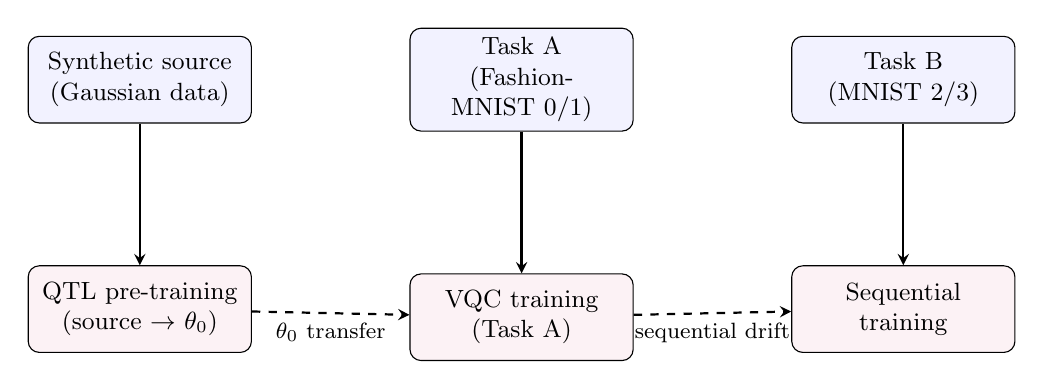
\begin{tikzpicture}[
  box/.style={draw, rectangle, minimum height=1.1cm, text width=2.6cm,
    align=center, fill=blue!05, rounded corners, font=\small},
  qbox/.style={draw, rectangle, minimum height=1.1cm, text width=2.6cm,
    align=center, fill=purple!05, rounded corners, font=\small},
  arrow/.style={thick,->,>=stealth}
]
  \node[box]  (src)   {Synthetic source\\(Gaussian data)};
  \node[box,  right=2.0cm of src]  (ta)   {Task A\\(Fashion-MNIST 0/1)};
  \node[box,  right=2.0cm of ta]   (tb)   {Task B\\(MNIST 2/3)};

  \node[qbox, below=1.8cm of src]  (pre)  {QTL pre-training\\(source $\rightarrow$ $\theta_0$)};
  \node[qbox, below=1.8cm of ta]   (vqa)  {VQC training\\(Task A)};
  \node[qbox, below=1.8cm of tb]   (seq)  {Sequential\\training};

  \draw[arrow] (src) -- (pre);
  \draw[arrow] (ta)  -- (vqa);
  \draw[arrow] (tb)  -- (seq);

  \draw[thick, dashed, ->, >=stealth] (pre) -- (vqa)
    node[midway, below, font=\footnotesize, align=center] {$\theta_0$ transfer};
  \draw[thick, dashed, ->, >=stealth] (vqa) -- (seq)
    node[midway, below, font=\footnotesize, align=center] {sequential drift};
\end{tikzpicture}%
}
\caption{Cross-domain QCL pipeline. Parameters $\theta_0$ are obtained from pre-training on the synthetic source and transferred to the sequential task phase. The dashed arrows represent weight initialization rather than data flow.}
\label{fig:pipeline}
\end{figure}

The hybrid model receives a four-dimensional input vector $x \in \mathbb{R}^4$ obtained from the dimensionality reduction stage. Real images first traverse a frozen MobileNetV2 backbone pre-trained on ImageNet, after which PCA maps the activations to four scalar features. The synthetic source is generated directly in $\mathbb{R}^4$ from synthetic Gaussian data. All inputs are linearly rescaled to the interval $[0, \pi]$ to match the rotation domain of the embedding layer. The classical-to-quantum interface follows Eq.~(1).

\begin{equation}
|\psi_{\text{in}}(x)\rangle = \bigotimes_{i=0}^{n-1} R_Y(x_i)\, |0\rangle^{\otimes n}
\end{equation}

where $n = 4$ is the number of qubits, $x_i$ is the $i$-th rescaled feature, $R_Y(\cdot)$ is the single-qubit rotation around the $Y$ axis, and $|0\rangle^{\otimes n}$ is the 4-qubit ground state.

The encoded quantum state propagates through a parameterized unitary $U(\theta)$ whose internal layout depends on the chosen ansatz. Three topologies are studied. The first is the Strongly Entangling Layers (SEL) block defined in Eq.~(2).

\begin{equation}
U_{\text{SEL}}(\theta) = \prod_{l=1}^{L} W_l \prod_{i=0}^{n-1} R(\theta_{l,i,1}, \theta_{l,i,2}, \theta_{l,i,3})
\end{equation}

where $L$ is the number of layers, $R(\alpha, \beta, \gamma)$ is the universal single-qubit rotation parameterized by three Euler angles, and $W_l$ is the cyclic CNOT entangler of layer $l$.

The second topology is the BE ansatz given in Eq.~(3). It applies a single rotation per qubit and per layer, which lowers the parameter count and the gate depth.

\begin{equation}
U_{\text{BE}}(\theta) = \prod_{l=1}^{L} W_l \prod_{i=0}^{n-1} R_X(\theta_{l,i})
\end{equation}

where $R_X(\cdot)$ is the rotation around the $X$ axis and $W_l$ is the cyclic CNOT entangler of Eq.~(2).

The third topology is the TTN, defined in Eq.~(4). The four wires are paired hierarchically. Each block applies one $R_Y$ and one $R_Z$ rotation followed by a CNOT, and the active wires combine towards qubits 0 and 1, where the readout occurs.

\begin{equation}
U_{\text{TTN}}(\theta) = \prod_{l=1}^{L} \prod_{b=0}^{n-2} \text{CNOT}_{i_b,j_b}\, R_Y(\theta_{l,b,1})_{i_b} \otimes R_Z(\theta_{l,b,2})_{j_b}
\end{equation}

where $b$ indexes the block, $(i_b, j_b)$ is the wire pair acted on by block $b$, and the product follows the hierarchical wiring of Figure 1.

The readout stage measures the expectation of the Pauli-$Z$ operator on the first two qubits as written in Eq.~(5).

\begin{equation}
z_k = \langle \psi_{\text{out}} | Z_k | \psi_{\text{out}} \rangle, \quad k \in \{0, 1\}
\end{equation}

where $|\psi_{\text{out}}\rangle = U(\theta)|\psi_{\text{in}}(x)\rangle$ and $Z_k$ is the Pauli-$Z$ operator acting on qubit $k$.

The two real-valued expectations $z_0$ and $z_1$ feed a fully connected classical layer that produces the binary logits as in Eq.~(6).

\begin{equation}
\hat{y} = W \begin{pmatrix} z_0 \\ z_1 \end{pmatrix} + b
\end{equation}

where $W \in \mathbb{R}^{2\times 2}$ and $b \in \mathbb{R}^{2}$ are trainable classical parameters and $\hat{y} \in \mathbb{R}^{2}$ are the unnormalized class scores. The training objective is the categorical cross-entropy of Eq.~(7). Predictions are obtained through the softmax normalization of $\hat{y}$.

\begin{equation}
L(\theta, W, b) = -\frac{1}{N} \sum_{i=1}^{N} \sum_{c=0}^{1} y_{i,c} \log \hat{p}_{i,c}
\end{equation}

where $N$ is the batch size, $y_{i,c}$ is the one-hot label of sample $i$ for class $c$, and $\hat{p}_{i,c}$ is the softmax probability obtained from $\hat{y}$.

The Cross-Domain Continual Learning protocol runs in three phases. The first phase pre-trains the full hybrid model on the source domain, either synthetic Gaussian or MobileNetV2 features, over fifteen epochs and stores the resulting parameters $\theta_0$ as the initialization for the subsequent CL stage. The second phase loads $\theta_0$ into a fresh model and trains on Task A, defined as Fashion-MNIST classes 0 and 1, over ten epochs. The third phase continues training on Task B, defined as MNIST classes 2 and 3, over ten further epochs. The forgetting drop is measured on the Task A test set after completion of the third phase. In Experiment 1, the lowest layer is frozen during the sequential phase and the learning rate is progressively reduced from 0.05 during the initial phase to 0.01 for Task A and 0.005 for Task B. This training schedule is applied identically to both the naive baseline and the synthetic QTL condition; the two conditions differ exclusively in the initialization of the circuit parameters $\theta_0$, which is random for the naive baseline and obtained from synthetic pre-training for the QTL condition. This design isolates the effect of the initialization strategy from any confound introduced by the freezing or the learning-rate schedule. Experiments 2 and 3 keep the full parameter set trainable under a constant learning rate to evaluate the influence of the circuit topology and the pre-training source.

Based on this protocol, three complementary experiments are conducted. Experiment 1 evaluates the effect of the proposed initialization protocol on CF under the experimental configuration described above. Experiment 2 analyzes the influence of circuit topology by comparing the SE, BE, and TTN ans\"atze under the same CL protocol. Experiment 3 evaluates the influence of the pre-training source on optimization behavior and target task performance by comparing scratch, synthetic QTL, and MobileNetV2 QTL initialization strategies.

The execution of the variational unitary on a real quantum processor is subject to gate errors and measurement readout errors that perturb the analytic state. To assess the robustness of the proposed protocol against this hardware reality, every experiment is replicated under three noise profiles. The first profile is the ideal one, where the unitary is propagated by the state-vector simulator without any error channel. The second and the third profiles route the circuit through a density-matrix simulator that interleaves a single-qubit depolarizing channel after every parameterized rotation, a two-qubit depolarizing channel after every CNOT, and a Pauli-$X$ bit-flip channel on every measured wire. Eq.~(8) defines the action of the depolarizing channel.

\begin{equation}
\mathcal{E}_{\text{dep}}(\rho) = (1-p)\rho + \frac{p}{3}\left( X\rho X + Y\rho Y + Z\rho Z \right)
\end{equation}

where $\rho$ is the input density matrix of the affected wire, $p$ is the depolarization probability, and $X$, $Y$, $Z$ are the single-qubit Pauli operators. The two-qubit version of Eq.~(8) is applied independently to each wire of the affected gate.

The bit-flip readout channel models the probability of recording the wrong measurement outcome. It is defined in Eq.~(9).

\begin{equation}
\mathcal{E}_{\text{ro}}(\rho) = (1-q)\rho + q\, X\rho X
\end{equation}

where $q$ is the readout error probability and $X$ is the Pauli-$X$ operator on the measured wire.

The first noise profile, called Heron r2, takes its parameters from the median calibration of the IBM Heron r2 generation of superconducting devices, with single-qubit depolarization $p = 3 \times 10^{-4}$, two-qubit depolarization $p = 3 \times 10^{-3}$ and readout error $q = 1.5 \times 10^{-2}$. The second noise profile, called Legacy NISQ, scales those parameters by approximately one order of magnitude towards the values reported on earlier generations such as IBM Eagle and Falcon devices, with single-qubit depolarization $p = 1 \times 10^{-3}$, two-qubit depolarization $p = 1.5 \times 10^{-2}$ and readout error $q = 3 \times 10^{-2}$.

To control the variance produced by the random initialization of the variational angles and by the stochastic optimization, the full pipeline is executed five times with independent random seeds in $\{0, 1, 2, 3, 4\}$ for each ansatz and each noise profile. All numerical results in Section IV are reported as the mean across the five seeds together with the population standard deviation. The factorial design of three noise profiles, three ans\"atze and five seed amounts to forty-five sequential trainings per experiment.

% ======================================================================
\section{Results}
% ======================================================================
This section reports the empirical analysis of the proposed protocol. The data sources are described first, followed by the formal metrics, the experimental configuration and the discussion of the three experiments stated in Section III.

\subsection{Data description}
Four data sources participate in the pipeline. The synthetic source produces Gaussian-cluster vectors using the \texttt{make\_classification} routine of scikit-learn with four informative features and two balanced classes. The CIFAR-10 source uses classes 2 (bird) and 3 (cat) of the standard split. Each image traverses a frozen MobileNetV2 backbone pre-trained on ImageNet, and the resulting feature vector is reduced to four principal components by PCA. Fashion-MNIST classes 0 (T-shirt/top) and 1 (Trouser) form Task A, and MNIST classes 2 and 3 form Task B. All inputs are rescaled to the interval $[0, \pi]$ to match the Angle Embedding domain. Table~\ref{tab:datasets} reports the sample counts used in the experiments.

\begin{table}[ht]
\caption{Sample counts per data source used in the experimental pipeline.}
\label{tab:datasets}
\centering
\begin{tabular}{llccc}
\toprule
Source & Role & Train & Test & Classes \\
\midrule
Synthetic (Gaussian) & QTL source & 2000 & 500 & 2 \\
CIFAR-10 (MobileNetV2) & QTL source & 1000 & 200 & 2, 3 \\
Fashion-MNIST & Task A & 1000 & 200 & 0, 1 \\
MNIST & Task B (target) & 1000 & 200 & 2, 3 \\
\bottomrule
\end{tabular}
\end{table}

\subsection{Metrics}
Three quantitative indicators capture the behavior of the model along the continual-learning protocol. The classification accuracy on a held-out test set is computed as in Eq.~(10).

\begin{equation}
\text{Acc} = \frac{1}{N} \sum_{i=1}^{N} \mathbb{I}(y_i = \hat{y}_i)
\end{equation}

where $N$ is the number of test samples, $y_i$ is the true label of sample $i$, $\hat{y}_i = \arg\max_c \hat{p}_{i,c}$ is the predicted label, and $\mathbb{I}(\cdot)$ is the indicator function.

The forgetting drop on Task A quantifies the accuracy lost on Task A after the sequential exposure to Task B as written in Eq.~(11).

\begin{equation}
\Delta_A = \text{Acc}_{A,\text{initial}} - \text{Acc}_{A,\text{final}}
\end{equation}

where $\text{Acc}_{A,\text{initial}}$ is the test accuracy on Task A measured immediately after the Task A training phase, and $\text{Acc}_{A,\text{final}}$ is the same accuracy measured after the Task B training phase. The third indicator is the per-epoch cross-entropy training loss already defined in Eq.~(7). It tracks the convergence speed on the target domain. Wall-clock training and inference times are also recorded as auxiliary cost indicators relevant for the NISQ context.

\subsection{Experimental Setup}
The pipeline runs on Python 3.11 over the Hercules supercomputing cluster of the Centro de Inform\'atica Cient\'ifica de Andaluc\'ia (CICA). Hercules comprises 232 compute nodes with a total of 11,136 CPU cores, 47.5 TB of RAM, and approximately 855 TFLOPS of peak performance, interconnected via a low-latency InfiniBand HDR network (200/100 Gbps). Jobs are managed using the SLURM workload manager. Experiments were executed on the standard partition using a single node equipped with four CPU cores and an NVIDIA A100 GPU (40 GB).

The software stack is composed of PennyLane 0.44.1 with the \texttt{default.qubit} simulator for the ideal profile and the \texttt{default.mixed} density matrix simulator for the noisy profiles, PyTorch 2.10.0, torchvision 0.25.0, scikit-learn 1.8.0, NumPy 2.4.3, and Matplotlib 3.10.8.

Each variational circuit operates over four qubits and three parameterized layers. The classical optimizer is Adam with a learning rate 0.05 in the source pre-training and Task A phases, 0.01 in the Task A fine-tuning of Experiment 1 and 0.005 in the Task B phase to protect the Task A representation. The batch size is 32 along the whole pipeline. The synthetic and MobileNetV2 sources train over fifteen epochs, and Tasks A and B train over ten epochs each. The cross-entropy criterion of PyTorch acts as the loss function. The random seed of scikit-learn is fixed at 42 to keep the synthetic generation reproducible. The noise profiles defined in Section III are activated at the simulator level, and each combination of profile, ansatz and seed runs as an independent task of an SLURM array on the cluster.

\subsection{Result Discussion}
The three experiments are first analyzed under the Heron r2 noise profile, which approximates the calibration of current superconducting hardware, and the comparison between the ideal and legacy NISQ profiles is reported at the end of the section to assess the robustness of the protocol to the noise level.

Experiment 1 evaluates the effect of the proposed initialization protocol on CF under the experimental configuration described in Section III. Table~\ref{tab:exp1} reports the forgetting drop $\Delta_A$ on Task A after the sequential training on Task B for the naive baseline and for the synthetic QTL initialization, averaged over five seeds and split by noise profile.

\begin{table}[ht]
\caption{Experiment 1. Forgetting drop $\Delta_A$ on Task A in percentage points (mean $\pm$ std over five seeds) per noise profile.}
\label{tab:exp1}
\centering
\begin{tabular}{lcc}
\toprule
Noise profile & Baseline $\Delta_A$ & QTL $\Delta_A$ \\
\midrule
Ideal & $72.10 \pm 2.33$ & $42.60 \pm 2.80$ \\
Heron r2 & $72.90 \pm 1.80$ & $44.10 \pm 3.34$ \\
Legacy NISQ & $70.50 \pm 6.43$ & $47.20 \pm 3.91$ \\
\bottomrule
\end{tabular}
\end{table}

Under the Heron r2 profile, the naive baseline loses, on average, 72.90 percentage points of Task A accuracy after exposure to Task B, whereas the synthetic QTL initialization reduces the forgetting drop to 44.10 percentage points. This corresponds to an absolute reduction of 28.80 percentage points. A similar trend is observed under the remaining noise profiles, where the forgetting drop decreases from 72.10 to 42.60 percentage points under the ideal profile and from 70.50 to 47.20 percentage points under the Legacy NISQ profile. These results indicate that the proposed initialization strategy substantially mitigates CF while maintaining its effectiveness under increasingly challenging noise conditions.

Experiment 2 evaluates the influence of circuit topology on task retention by comparing the three parameterized quantum circuit ans\"atze under the same CL protocol. Table~\ref{tab:exp2time} reports, for the Heron r2 noise profile, the final Task A and Task B accuracies for the SE, BE, and TTN architectures together with the corresponding wall-clock training and inference times, allowing the retention capability of each topology to be interpreted together with its computational cost. Wall-clock times are reported only for the Heron r2 profile, as it is calibrated to the current generation of superconducting hardware and therefore constitutes the most representative case for assessing computational cost in a realistic NISQ deployment. The ideal profile, simulated with the state-vector \texttt{default.qubit} backend, is computationally cheaper, as it avoids the overhead of the density-matrix simulation. The Legacy NISQ profile, simulated under the same density-matrix \texttt{default.mixed} backend as Heron r2, exhibits comparable wall-clock cost.

\begin{table}[ht]
\caption{Experiment 2 under the Heron r2 noise profile. Training and inference times (in seconds) together with the final accuracies (in \%) on Tasks A and B (mean $\pm$ std over five seeds, standard deviation reported only for accuracies).}
\label{tab:exp2time}
\centering
\begin{tabular}{lcccccc}
\toprule
Ansatz & Tr. A & Tst. A & Acc. A & Tr. B & Tst. B & Acc. B \\
\midrule
SE & 45.26 & 0.61 & $96.50 \pm 0.55$ & 51.25 & 0.61 & $89.60 \pm 1.02$ \\
BE & 41.45 & 0.57 & $73.10 \pm 1.20$ & 46.90 & 0.57 & $58.20 \pm 2.11$ \\
TTN & 42.18 & 0.56 & $95.40 \pm 1.39$ & 47.91 & 0.56 & $89.80 \pm 0.60$ \\
\bottomrule
\end{tabular}
\end{table}

The SE ansatz reaches 96.50\% on Task A and 89.60\% on Task B, indicating that it maintains a high level of performance after the sequential learning process. The BE exhibits the lowest performance, reaching 73.10\% on Task A and 58.20\% on Task B. In contrast, the TTN achieves 95.40\% on Task A and 89.80\% on Task B while requiring a slightly lower wall-clock training time than the SE architecture. Under the evaluated conditions, both the SE and TTN ans\"atze achieve substantially higher Task A accuracy after sequential training than the BE, at a comparable or lower computational cost.

Table~\ref{tab:exp2acc} extends the comparison to the three evaluated noise profiles. The SE and TTN ans\"atze consistently maintain Task A accuracies above 95\%, whereas the BE remains below 74\% in all three profiles. In addition, the ranking among the three ans\"atze is preserved under the ideal, Heron r2, and Legacy NISQ profiles, indicating that the observed differences remain consistent under the evaluated noise conditions. The standard deviation of the SE ansatz also decreases slightly from 0.81 under the ideal profile to 0.51 under the Legacy NISQ profile, although further experiments would be required to determine the origin of this behavior.

\begin{table}[ht]
\caption{Experiment 2. Final Task A accuracy (\%) after sequential training on Task B under the three evaluated noise profiles (mean $\pm$ std over five seeds).}
\label{tab:exp2acc}
\centering
\begin{tabular}{lccc}
\toprule
Noise Profile & SE & BE & TTN \\
\midrule
Ideal & $96.30 \pm 0.81$ & $72.90 \pm 1.36$ & $95.40 \pm 1.39$ \\
Heron r2 & $96.50 \pm 0.55$ & $73.10 \pm 1.20$ & $95.40 \pm 1.39$ \\
Legacy NISQ & $96.70 \pm 0.51$ & $72.30 \pm 0.81$ & $95.30 \pm 1.08$ \\
\bottomrule
\end{tabular}
\end{table}

Experiment 3 evaluates the influence of the pre-training source on optimization behavior and target task performance under three initialization strategies: random initialization (scratch), synthetic QTL, and MobileNetV2 QTL. Figure~\ref{fig:exp3} compares the evolution of the cross-entropy loss during target training for the three initialization strategies. Solid curves represent the mean over five random seeds, while the shaded regions indicate one standard deviation. Lower curves indicate faster convergence. Table~\ref{tab:exp3time} complements this analysis by reporting the corresponding training and inference times (in seconds) together with the final target accuracy (in \%).

\begin{figure}[ht]
\centering
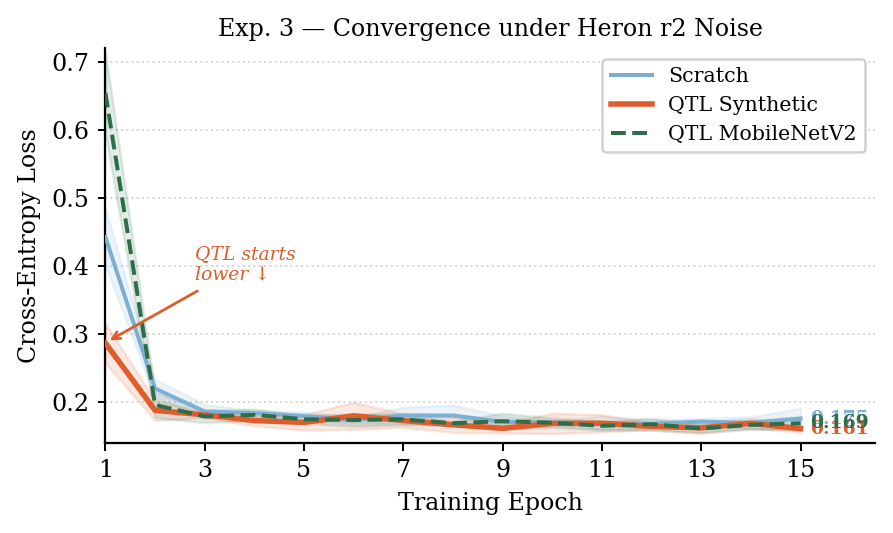
\includegraphics[width=\linewidth]{figures/fig2_exp3_convergence.png}
\caption{Experiment 3. Cross-entropy loss during target training under the Heron r2 noise profile.}
\label{fig:exp3}
\end{figure}

\begin{table}[ht]
\caption{Experiment 3 under the Heron r2 noise profile. Wall-clock cost and final test accuracy on the MNIST target for each initialization paradigm (mean $\pm$ std over five seeds, std reported on the accuracy).}
\label{tab:exp3time}
\centering
\begin{tabular}{lccc}
\toprule
Initialization Strategy & Train Time & Test Time & Target Acc. \\
\midrule
Pre-Training Source (Synthetic) & 134.21 & 1.41 & $83.60 \pm 1.23$ \\
Pre-Training Source (MobileNetV2) & 68.00 & 0.61 & $83.40 \pm 2.60$ \\
Target Training (Scratch) & 67.69 & 0.60 & $90.80 \pm 1.54$ \\
Target Training (QTL Synthetic) & 67.85 & 0.61 & $89.90 \pm 0.58$ \\
Target Training (QTL MobileNetV2) & 67.56 & 0.60 & $88.60 \pm 1.36$ \\
\bottomrule
\end{tabular}
\end{table}

The three initialization strategies reach a comparable accuracy plateau on the MNIST target. The scratch baseline reaches 90.80\%, the synthetic QTL initialization reaches 89.90\%, and the MobileNetV2 QTL initialization reaches 88.60\%. The synthetic QTL initialization also exhibits lower variability across the evaluated seeds, with a standard deviation of 0.58 percentage points compared with 1.54 for the scratch baseline. The training time of the QTL-based initialization strategies differs by less than one second from the scratch baseline during the target training phase, while the inference time remains close to 0.60 seconds per test set.

Table~\ref{tab:exp3acc} reports the target accuracy under the three evaluated noise profiles. The accuracy remains within a 1.5-percentage-point interval for all profiles and initialization strategies, indicating that the different initialization strategies have only a limited impact on the final target accuracy. Under the Legacy NISQ profile, the three initialization strategies converge to very similar accuracies (89.60\%, 89.90\%, and 89.70\%, respectively), suggesting that the higher gate error partially reduces the differences introduced by the initialization while the synthetic QTL initialization still exhibits lower variability across seeds ($\sigma = 1.24$ versus $\sigma = 2.33$ for the scratch baseline). Under the ideal profile, the synthetic QTL initialization slightly surpasses the scratch baseline (90.90\% versus 90.10\%), although the difference remains small.

\begin{table}[ht]
\caption{Experiment 3 --- target accuracy (\%) per initialization paradigm across noise profiles (mean $\pm$ std over five seeds).}
\label{tab:exp3acc}
\centering
\begin{tabular}{lccc}
\toprule
Noise Profile & Scratch & QTL-Syn & QTL-Mob \\
\midrule
Ideal & $90.10 \pm 1.91$ & $90.90 \pm 1.43$ & $89.70 \pm 1.03$ \\
Heron r2 & $90.80 \pm 1.54$ & $89.90 \pm 0.58$ & $88.60 \pm 1.36$ \\
Legacy NISQ & $89.60 \pm 2.33$ & $89.90 \pm 1.24$ & $89.70 \pm 1.54$ \\
\bottomrule
\end{tabular}
\end{table}

% ======================================================================
\section{Conclusions}
% ======================================================================
This work investigated the use of cross-domain synthetic pre-training as a memory-free initialization strategy for QCL in hybrid quantum-classical models. The proposed protocol has been evaluated using five random seeds and three noise profiles representing an ideal state-vector simulator, the calibration of the IBM Heron r2 generation, and a legacy NISQ regime with higher gate and readout error. Under the Heron r2 profile, the synthetic pre-training strategy reduces the forgetting drop on Task A from $72.90 \pm 1.80$ to $44.10 \pm 3.34$ percentage points, corresponding to an absolute reduction of 28.80 percentage points. Comparable improvements are also observed under the ideal profile, with a reduction of 29.50 points, and under the Legacy NISQ profile, with a reduction of 23.30 points, indicating that the proposed initialization strategy consistently reduces forgetting under the evaluated noise conditions. The comparison of the three circuit topologies shows that the SE and TTN architectures consistently achieve higher Task A accuracy after sequential training than the BE, while the comparison of the three initialization strategies indicates that synthetic QTL, MobileNetV2 QTL, and scratch initialization reach comparable target accuracies within a 1.5-percentage-point interval, with the synthetic initialization exhibiting lower variability across random seeds. Although the proposed approach consistently improves knowledge retention, the experiments also show that CF is not completely eliminated in the evaluated four-qubit setting and that the initialization strategy does not produce a significant increase in the final target-task accuracy. These results suggest that cross-domain synthetic pre-training constitutes a useful complementary mechanism rather than a complete solution to CF. Future work will investigate the scalability of the proposed approach to larger quantum circuits and deeper ans\"atze, evaluate alternative dimensionality reduction strategies beyond PCA, study its combination with established CL methods such as parameter-space regularization, and validate the proposed methodology on real superconducting quantum hardware.

\section*{Acknowledgment}
The authors would like to thank the Spanish Ministry of Science and Innovation and Pablo de Olavide University for the support within the projects PID2023-146037OB-C22 and PPI2505. The authors also acknowledge the Junta de Andaluc\'ia's Centro de Inform\'atica Cient\'ifica de Andaluc\'ia (CICA) for providing the computing resources on the H\'ercules supercomputer, which were instrumental in performing the simulations/calculations presented in this work.

% NOTE: figure 1 (pipeline) is drawn with TikZ in the Methodology section.

\begin{thebibliography}{00}
\bibitem{b1} F. Rodr\'iguez-D\'iaz, D. Guti\'errez-Avil\'es, A. Troncoso, and F. Mart\'inez-\'Alvarez, ``A survey of quantum machine learning: Foundations, algorithms, frameworks, data and applications,'' \emph{ACM Computing Surveys}, vol. 58, p. 91, 2026.
\bibitem{b2} M. Cerezo, A. Arrasmith, R. Babbush, S. C. Benjamin, S. Endo, K. Fujii, J. R. McClean, K. Mitarai, X. Yuan, L. Bozhedarov, \emph{et al.}, ``Variational quantum algorithms,'' \emph{Nature Reviews Physics}, vol. 3, no. 9, pp. 625--644, 2021.
\bibitem{b3} G. I. Parisi, R. Kemker, J. L. Part, C. Kanan, and S. Wermter, ``Continual lifelong learning with neural networks: A review,'' \emph{Neural Networks}, vol. 113, pp. 54--71, 2019.
\bibitem{b4} P. Buzzega, M. Boschini, A. Porrello, D. Abati, and S. Calderara, ``Dark experience for general continual learning: a strong, simple baseline,'' in \emph{Advances in Neural Information Processing Systems}, vol. 33, pp. 15920--15930, 2020.
\bibitem{b5} J. Kirkpatrick, R. Pascanu, N. Rabinowitz, J. Veness, G. Desjardins, A. A. Rusu, K. Milan, J. Quan, T. Ramalho, A. Grabska-Barwinska, \emph{et al.}, ``Overcoming catastrophic forgetting in neural networks,'' \emph{Proceedings of the National Academy of Sciences}, vol. 114, no. 13, pp. 3521--3526, 2017.
\bibitem{b6} A. Pesah, M. Cerezo, S. Wang, T. Volkoff, A. Sone, and P. J. Coles, ``Absence of barren plateaus in quantum convolutional neural networks,'' \emph{Physical Review X}, vol. 11, no. 4, p. 041011, 2021.
\bibitem{b7} D. Mart\'in-P\'erez, F. Rodr\'iguez-D\'iaz, D. Guti\'errez-Avil\'es, A. Troncoso, and F. Mart\'inez-\'Alvarez, ``Hybrid classical-quantum transfer learning with noisy quantum circuits,'' \emph{Computer Modeling in Engineering and Sciences}, vol. 147, p. 82712, 2026.
\bibitem{b8} A. Mari, T. R. Bromley, J. Izaac, M. Schuld, and N. Killoran, ``Transfer learning in hybrid classical-quantum neural networks,'' \emph{Quantum}, vol. 4, p. 340, 2020.
\bibitem{b9} S. J. Pan and Q. Yang, ``A survey on transfer learning,'' \emph{IEEE Transactions on Knowledge and Data Engineering}, vol. 22, no. 10, pp. 1345--1359, 2009.
\bibitem{b10} D. Mart\'in-P\'erez, F. Rodr\'iguez-D\'iaz, A. Troncoso, and F. Mart\'inez-\'Alvarez, ``Mitigating catastrophic forgetting in quantum neural networks via hybrid topologies and dark experience replay,'' \emph{Communications in Computer and Information Science}, vol. 3046, pp. 463--472, 2026.
\bibitem{b11} H. Xiao, K. Rasul, and R. Vollgraf, ``Fashion-MNIST: a Novel Image Dataset for Benchmarking Machine Learning Algorithms,'' \emph{arXiv preprint arXiv:1708.07747}, 2017.
\bibitem{b12} Y. Lecun, L. Bottou, Y. Bengio, and P. Haffner, ``Gradient-based learning applied to document recognition,'' \emph{Proceedings of the IEEE}, vol. 86, no. 11, pp. 2278--2324, 1998.
\bibitem{b13} M. Sandler, A. Howard, M. Zhu, A. Zhmoginov, and L. C. Chen, ``MobileNetV2: Inverted Residuals and Linear Bottlenecks,'' in \emph{Proceedings of the IEEE Conference on Computer Vision and Pattern Recognition}, pp. 4510--4520, 2018.
\bibitem{b14} S. Sim, P. D. Johnson, and A. Aspuru-Guzik, ``Expressibility and entangling capability of parameterized quantum circuits for hybrid quantum-classical algorithms,'' \emph{Advanced Quantum Technologies}, vol. 2, no. 12, p. 1900070, 2019.
\bibitem{b15} E. Grant, M. Benedetti, S. Cao, A. Hallam, J. Lockhart, T. Vidick, S. Severini, and L. Oswald, ``Hierarchical quantum classifiers,'' \emph{npj Quantum Information}, vol. 4, no. 1, p. 65, 2018.
\bibitem{b16} M. McCloskey and N. J. Cohen, ``Catastrophic Interference in Connectionist Networks: The Sequential Learning Problem,'' \emph{Psychology of Learning and Motivation}, vol. 24, pp. 109--165, 1989.
\bibitem{b17} R. Hadsell, D. Rao, A. A. Rusu, and R. Pascanu, ``Embracing Change: Continual Learning in Deep Neural Networks,'' \emph{Trends in Cognitive Sciences}, vol. 24, no. 12, pp. 1028--1040, 2020.
\bibitem{b18} M. De Lange, R. Aljundil, M. Masana, S. Parisot, X. Jia, and A. Leonardis, ``A Continual Learning Survey: Defying Forgetting in Classification Tasks,'' \emph{IEEE Transactions on Pattern Analysis and Machine Intelligence}, vol. 44, no. 7, pp. 3366--3385, 2022.
\bibitem{b19} F. Zenke, B. Poole, and S. Ganguli, ``Continual Learning Through Synaptic Intelligence,'' \emph{arXiv preprint arXiv:1703.04200}, 2017.
\bibitem{b20} Z. Li and D. Hoiem, ``Learning without Forgetting,'' \emph{IEEE Transactions on Pattern Analysis and Machine Intelligence}, vol. 40, no. 12, pp. 2935--2947, 2018.
\bibitem{b21} S. A. Rebuffi, A. Kolesnikov, G. Sperl, and C. H. Lampert, ``iCaRL: Incremental Classifier and Representation Learning,'' in \emph{Proceedings of the IEEE Conference on Computer Vision and Pattern Recognition}, pp. 5533--5542, 2017.
\bibitem{b22} G. M. van de Ven, T. Tuytelaars, and A. S. Tolias, ``Three types of incremental learning,'' \emph{Nature Machine Intelligence}, vol. 4, pp. 1185--1197, 2022.
\bibitem{b23} J. Preskill, ``Quantum Computing in the NISQ era and beyond,'' \emph{Quantum}, vol. 2, p. 79, 2018.
\bibitem{b24} K. Sharma, M. Cerezo, L. Cincio, and P. J. Coles, ``Trainability of Dissipative Perceptron-Based Quantum Neural Networks,'' \emph{Physical Review Letters}, vol. 128, 2022.
\bibitem{b25} S. Wang, E. Fontana, M. Cerezo, K. Sharma, A. Sone, L. Cincio, and P. J. Coles, ``Noise-induced barren plateaus in variational quantum algorithms,'' \emph{Nature Communications}, vol. 12, no. 6961, 2021.
\bibitem{b26} C. Zhang, Z. Lu, L. Zhao, S. Xu, W. Li, \emph{et al.}, ``Experimental demonstration of quantum continual learning with superconducting qubits,'' \emph{npj Quantum Information}, vol. 12, no. 28, 2026.
\bibitem{b27} J. Yosinski, J. Clune, Y. Bengio, and H. Lipson, ``How transferable are features in deep neural networks?,'' \emph{Advances in Neural Information Processing Systems}, vol. 27, 2014.
\bibitem{b28} A. Skolik, J. R. McClean, M. Mohseni, P. van der Smagt, and M. Leib, ``Layerwise learning for quantum neural networks,'' \emph{Quantum Machine Intelligence}, vol. 3, no. 5, 2021.
\end{thebibliography}

\end{document}
